%%% LaTeX Template: Two column article
%%%
%%% Source: http://www.howtotex.com/
%%% Feel free to distribute this template, but please keep to referal to http://www.howtotex.com/ here.
%%% Date: February 2011

%%% Preamble
\documentclass[	DIV=calc,%
							paper=a4,%
							fontsize=12pt,%
							onecolumn]{scrartcl}	 					% KOMA-article class

\usepackage{lipsum}													% Package to create dummy text
\usepackage[brazil]{babel}										% English language/hyphenation
\usepackage[protrusion=true,expansion=true]{microtype}				% Better typography
\usepackage{amsmath,amsfonts,amsthm}					% Math packages
\usepackage[pdftex]{graphicx}									% Enable pdflatex
\usepackage[svgnames]{xcolor}									% Enabling colors by their 'svgnames'
\usepackage[hang, small,labelfont=bf,up,textfont=it,up]{caption}	% Custom captions under/above floats
\usepackage{epstopdf}												% Converts .eps to .pdf
\usepackage{subfig}													% Subfigures
\usepackage{booktabs}												% Nicer tables
\usepackage{fix-cm}													% Custom fontsizes
\usepackage[utf8]{inputenc}
\usepackage[top=2.5cm, bottom=2.5cm, left=2.5cm, right=2.5cm]{geometry}
\usepackage[ddmmyyyy]{datetime}
\addto\captionsenglish{%
	\renewcommand\tablename{Tabela}
	\renewcommand\figurename{Figura}
} 
 

 
%%% Custom sectioning (sectsty package)
\usepackage{sectsty}													% Custom sectioning (see below)
\allsectionsfont{%															% Change font of al section commands
	\usefont{OT1}{phv}{b}{n}%										% bch-b-n: CharterBT-Bold font
	}

\sectionfont{%																% Change font of \section command
	\usefont{OT1}{phv}{b}{n}%										% bch-b-n: CharterBT-Bold font
	}



%%% Headers and footers
\usepackage{fancyhdr}												% Needed to define custom headers/footers
	\pagestyle{fancy}														% Enabling the custom headers/footers
\usepackage{lastpage}	

% Header (empty)
\lhead{}
\chead{}
\rhead{}
% Footer (you may change this to your own needs)

%% ====================================
%% ====================================
%% mude o rodape  do projeto
%% ====================================
%% ====================================

\lfoot{\footnotesize \texttt{Template para entrega de texto} \textbullet ~Modelo de projeto}


\cfoot{}
\rfoot{\footnotesize página \thepage\ de \pageref{LastPage}}	% "Page 1 of 2"
\renewcommand{\headrulewidth}{0.0pt}
\renewcommand{\footrulewidth}{0.4pt}



%%% Creating an initial of the very first character of the content
\usepackage{lettrine}
\newcommand{\initial}[1]{%
     \lettrine[lines=3,lhang=0.3,nindent=0em]{
     				\color{DarkGoldenrod}
     				{\textsf{#1}}}{}}



%%% Title, author and date metadata
\usepackage{titling}															% For custom titles

\newcommand{\HorRule}{\color{DarkGoldenrod}%			% Creating a horizontal rule
									  	\rule{\linewidth}{1pt}%
										}

\pretitle{\vspace{-30pt} \begin{flushleft} \HorRule 
				\fontsize{50}{50} \usefont{OT1}{phv}{b}{n} \color{DarkRed} \selectfont 
				}

%% ====================================
%% ====================================
%% mude o titulo  do projeto
%% ====================================
%% ====================================

\title{Modelo para Relatório individual e projeto}					% Title of your article goes here

%% ====================================



\posttitle{\par\end{flushleft}\vskip 0.5em}

\preauthor{\begin{flushleft}
					\large \lineskip 0.5em \usefont{OT1}{phv}{b}{sl} \color{DarkRed}}
\author{Alexandre L'Erario, Adan Matsudo, Antônio Henrique, Camila Gonçalves, Danillo Lima, Guilherme Tavares.}  	% Author name goes here


\postauthor{\footnotesize \usefont{OT1}{phv}{m}{sl} \color{Black} 
					\\Universidade Tecnológica Federal do Paraná - Câmpus Cornélio Procópio 								% Institution of author
					\par\end{flushleft}\HorRule}

\date{}																				% No date




%%% Begin document
\begin{document}
\maketitle
\thispagestyle{fancy} 	
\thispagestyle{empty}		% Enabling the custom headers/footers for the first page 
% The first character should be within \initial{}




%% ====================================
%% ====================================
%% mude o resumo  do projeto
%% ====================================
%% ====================================
\initial{O}\textbf{ processo de desenvolvimento proposto é iterativo e incremental e possui onze etapas. Cada uma das etapas possuem um documento de entrada e a partir dele é gerado um documento de saída que mapeia todo o processo de desenvolvimento. Ao final de cada ciclo/iteração é entregue uma versão funcional do sistema até que seja implementadas todos as tarefas, após isso é entregue a versão final do sistema.}

%% ====================================
\begin{figure}
	\centering
	
\includegraphics{utfpr}
\end{figure}

\vspace{3cm}
\centerline{\textit{\textbf{\today}}}

\clearpage
    \renewcommand*\listfigurename{Lista de figuras}
\listoffigures

\renewcommand*\listtablename{Lista de tabelas}
\listoftables




\clearpage
\renewcommand{\contentsname}{Sumário}
\tableofcontents
\clearpage

%% ====================================
%% ====================================
%% Inicio do texto
%% ====================================
%% ====================================
\section{Introdução}
 O processo PIEI - Processo Iterativo e Incremental se inicia com o levantamento de requisitos, onde é feito uma entrevista com o usuário para identificar suas necessidades e transforma-lás em atividades que sejam solucionáveis de forma computacional, a partir da entrevista é registrado as histórias de usuário onde, então, será gerado as atividades para a construção do sistema. 
 
 Após a definição das atividades, estas serão priorizadas de acordo a necessidade do cliente e dependências de outras atividades. Uma vez que as atividades foram priorizadas, algumas serão selecionadas para que caibam em um período de execução de 15 a 20 dias, então segue-se com a reunião de planejamento onde será definido o que é necessário fazer em cada uma das tarefas assim a equipe de desenvolvimento já poderá estimar cada uma das tarefas de acordo com a base histórica. Uma vez que as atividades que foram estimadas caibam na execução da iteração segue-se com a implementação das atividades. Durante a implementação também será escrito os test cases, que serão executados, e também deve ser documentado a funcionalidade que será entregue.Ao final da apresentação deve-se realizar uma apresentação das funcionalidades implementadas ao cliente e preenchido a base histórica. 
 
 Após a apresentação toda a equipe irá fazer uma retrospectiva e apontar os pontos que precisam, melhorar, parar e manter. Após a retrospectiva será entregue uma versão funcional do sistema ao cliente e então o processo se reinicia a até ser entregue a versão final do sistema. O projeto foi feito Antônio Henrique Cícero, Camila de Souza Gonçalves, Danillo Lima, Guilherme T. Tempesta, Adan Matsudo.
 
\section{Processo}
Descreva aqui o processo utilizado.

\subsection{Papeis}
Explique e enumere os papeis (roles) do processo.

\begin{itemize}
	\item Cliente: Define os requisitos do produto que será utilizado no processo, e o que é importante no produto de software.
	\item Analista de Software: Levanta requisitos claros e concisos, verificam por conflitos, define o  escopo de sistemas novos e como será as modificações nos sistemas já existentes.
	\item Desenvolvedor: Responsáveis pela parte técnica do programa, no final de cada atividade as funcionalidades. 
	\item Gerente de Projetos: Acompanha a execução do projeto. 
\end{itemize}

\subsection{Atividades}
Enumere e explique cada uma das atividades, relacione com os papéis.
\begin{itemize}
	\item \textbf{Levantamento de requisitos}
	\subitem Artefatos de entrada: Questionário e perguntas dissertativas pré-estabelecidas
	\subitem Descrição: O analista registra o dialogo com o cliente, faz anotações e usa um questionário padronizado para levantar as funcionalidades juntamente com uma descrição delas e do software final, com o cliente, o analista também tenta perceber se existe conflitos, inviabilidade e/ou impossibilidades nos requisitos descritos até então.
	\subitem Artefatos de saída: Formulários de requisitos funcionais e não funcionais	
	\item \textbf{Definir tarefas com base nos requisitos}
	\subitem Artefatos de entrada: Formulários de requisitos funcionais e não funcionais
	\subitem Descrição: Com base no questionário e anotações anteriores o analista e os desenvolvedores analisam os requisitos e tentam quebra-los em tarefas necessárias para entregar essas funcionalidades.
	\subitem Artefatos de saída: Documento com definição das tarefas

	\item Priorizar tarefas: 
	\subitem Artefatos de entrada: Documento com definição das tarefas
	\subitem Descrição: 
	Após tarefas estabelecidas, cabe ao gerente de projeto definir as prioridades de desenvolvimento.
	\subitem Artefatos de saída: Documento definindo um grau de prioridade para cada tarefa

	\item Definir tarefas da iteração: 
	\subitem Artefatos de entrada: Documento definindo um grau de prioridade para cada tarefa
	\subitem Descrição: Com base na prioridade das tarefas, é determinado quais serão executadas de acordo com uma sequência estipulada. 
	\subitem Artefatos de saída: Documento definindo tarefas que serão feitas por iteração
	
	\item Reunião de planejamento: confecção de protótipo
	\subitem Artefatos de entrada: Documento definindo tarefas por interação
	\subitem Descrição: 
	A reunião é descrito o que precisa ser feito em cada tarefa e deve ser realizado um protótipo, caso necessário.
	\subitem Artefatos de saída: Documento de proposta de reunião
	
	\item Estimar Tarefas:  
	\subitem Artefatos de entrada: Base histórica(Quando houver), Documento de tarefas
	\subitem Descrição: A estimativa das tarefas são estabelecidas de acordo com o tempo em que serão executada (Utilizando base histórica).
	\subitem Artefatos de saída: 
	
	\item Implementação: 
	\subitem Artefatos de entrada: Documento de requisitos e documento de tarefas da iteração 
	\subitem Descrição: Nesta fase é o momento em que desenvolvedor elabora o que na atividade estipulado. Cada desenvolvedor precisa escrever um test case para sua tarefa e outro desenvolvedor deve testa-lá. Documentar cada funcionalidade gerada a partir das tarefas entregues.
	\subitem Artefatos de saída: Linhas de código 
	
	\item Apresentar Funcionalidades: 
	\subitem Artefatos de entrada: Linhas de código e 
	\subitem Descrição: Em seguida, é feita uma reunião onde serão exibidos os “produtos” gerados pela iteração. 
	\subitem Artefatos de saída: Build do software e documento descrevendo os requisitos implementados. 
	
	\item Retrospectiva: 
	\subitem Artefatos de entrada:
	\subitem Descrição: Uma reunião é realizada de modo que apresente os resultados do produto e como foi realizado a sua evolução, focando principalmente em pontos que podem ser melhorados.
	\subitem Artefatos de saída:
\end{itemize}


\section{Execução do projeto}

Relacione as atividades com os integrantes, crie um cronograma conforme orientações
\subsection{Backlog e sprints}
-- item obrigatório --

Evidencie todos os stakeholders involvidos


\subsection{Estado atual}
Artefatos gerados em ordem cronológica, conforme processo. 
\begin{enumerate}
	\item Documentos de requisitos funcionais e não funcionais (Figuras \ref{Figura 1}, \ref{Figura 2})
	\item Documento de definição de tarefas e de priorização(Figura \ref{Figura 3})
	\item Distribuição de tarefas por iteração
\end{enumerate}

\begin{figure}
	\centering
	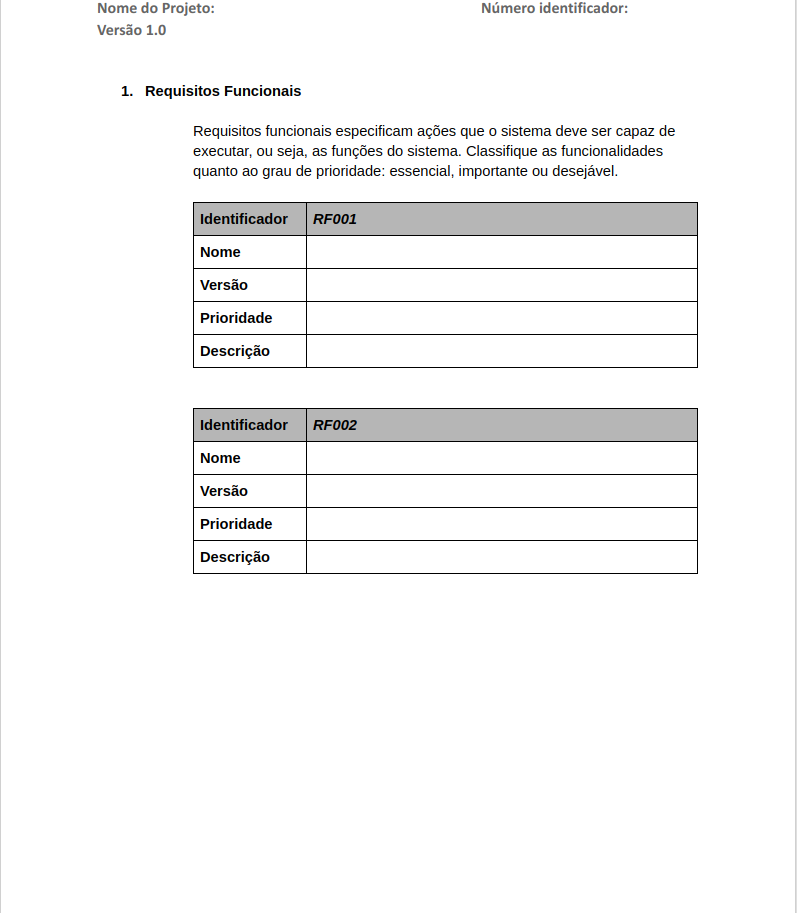
\includegraphics[width=\textwidth]{requisitos1}
	\caption{Formulário de requisitos funcionais}
	\label{Figura 1}
\end{figure}

\begin{figure}
	\centering
	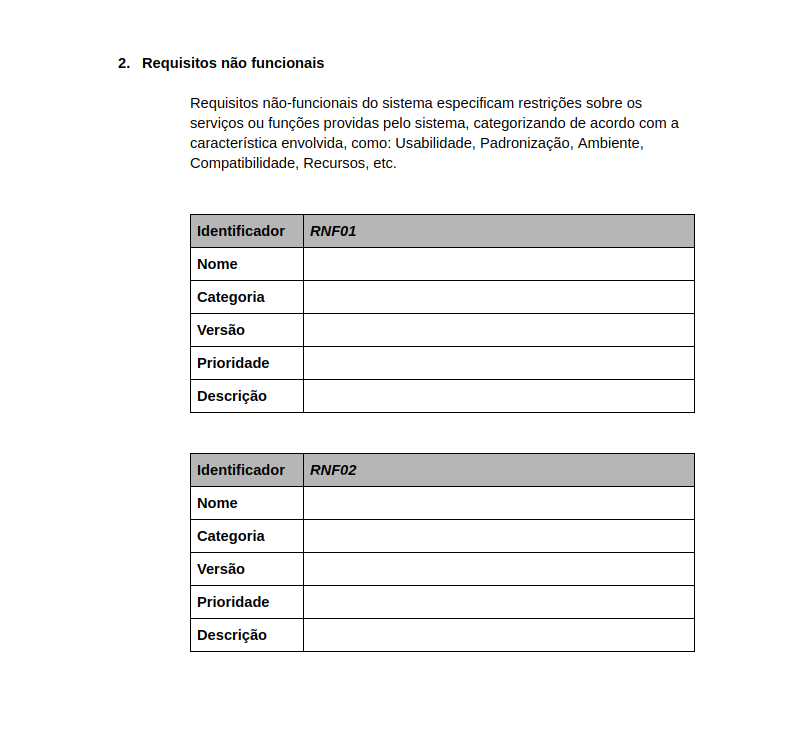
\includegraphics[width=\textwidth]{requisitos2}
	\caption{Formulário requisitos não funcionais}
	\label{Figura 2}
\end{figure}

\begin{figure}
	\centering
	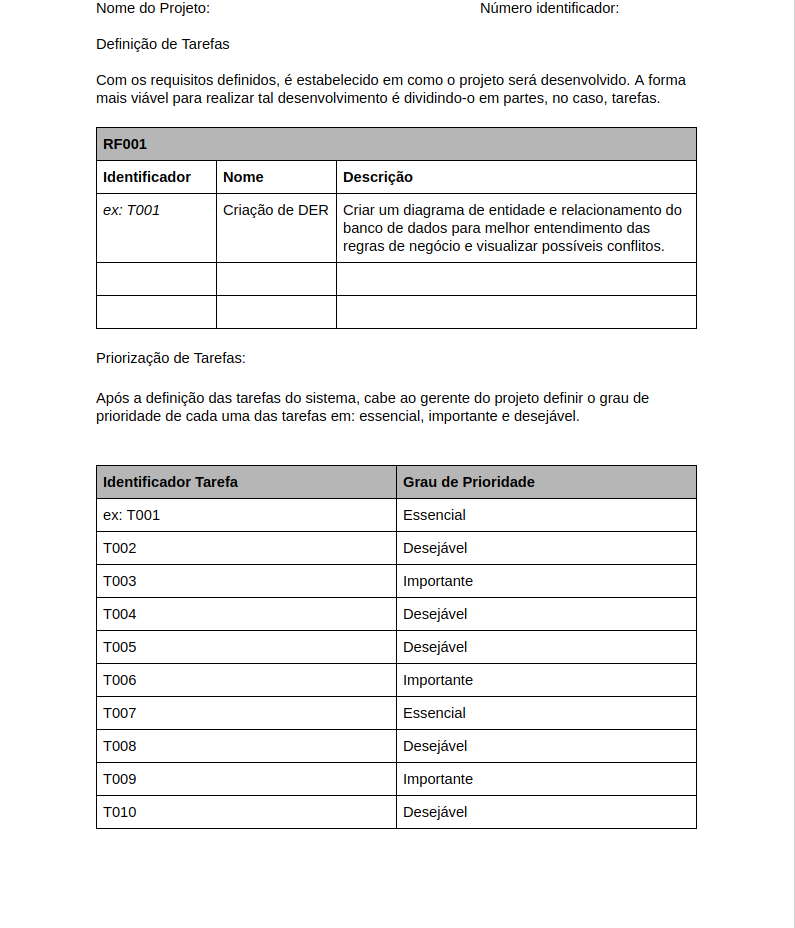
\includegraphics[width=\textwidth]{tarefas1}
	\caption{Formulários de definição e priorização de tarefas}
	\label{Figura 3}
\end{figure}

\begin{figure}
	\centering
	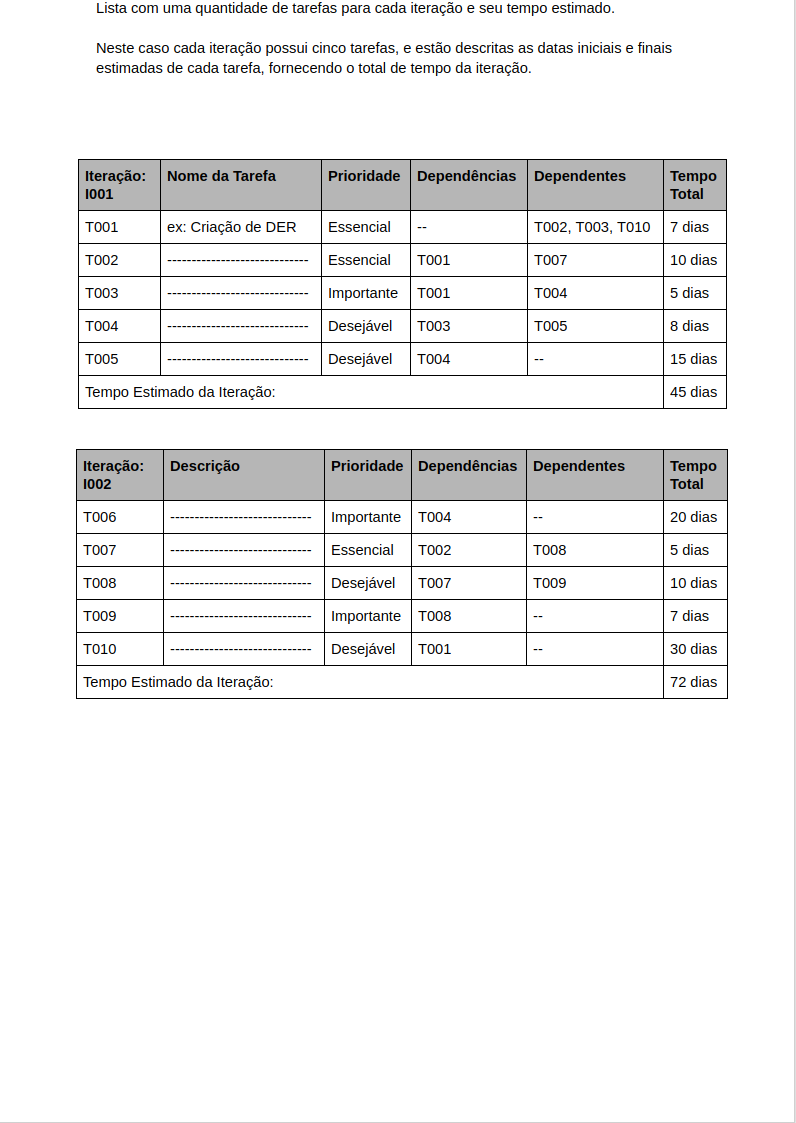
\includegraphics[width=\textwidth]{tarefas2}
	\caption{Lista com nome das tarefas designado para cada iteração}
	\label{Figura 4}
\end{figure}


\begin{figure}
	\centering
	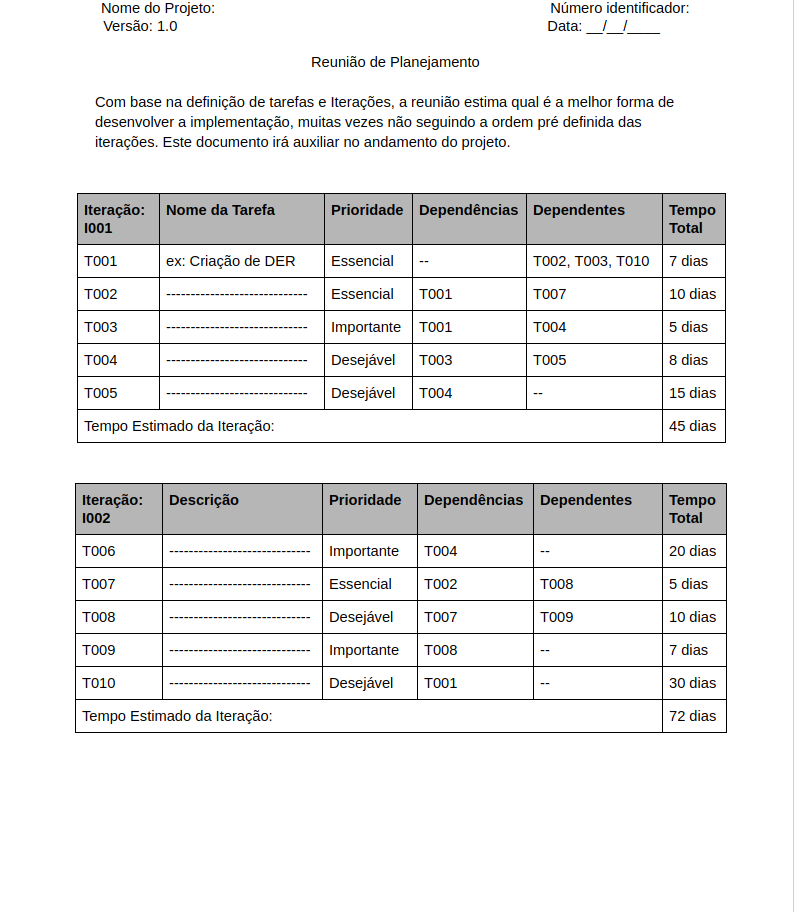
\includegraphics[width=\textwidth]{planejamento1}
	\caption{Reunião de planejamento}
	\label{Figura 5}
\end{figure}


\begin{figure}
	\centering
	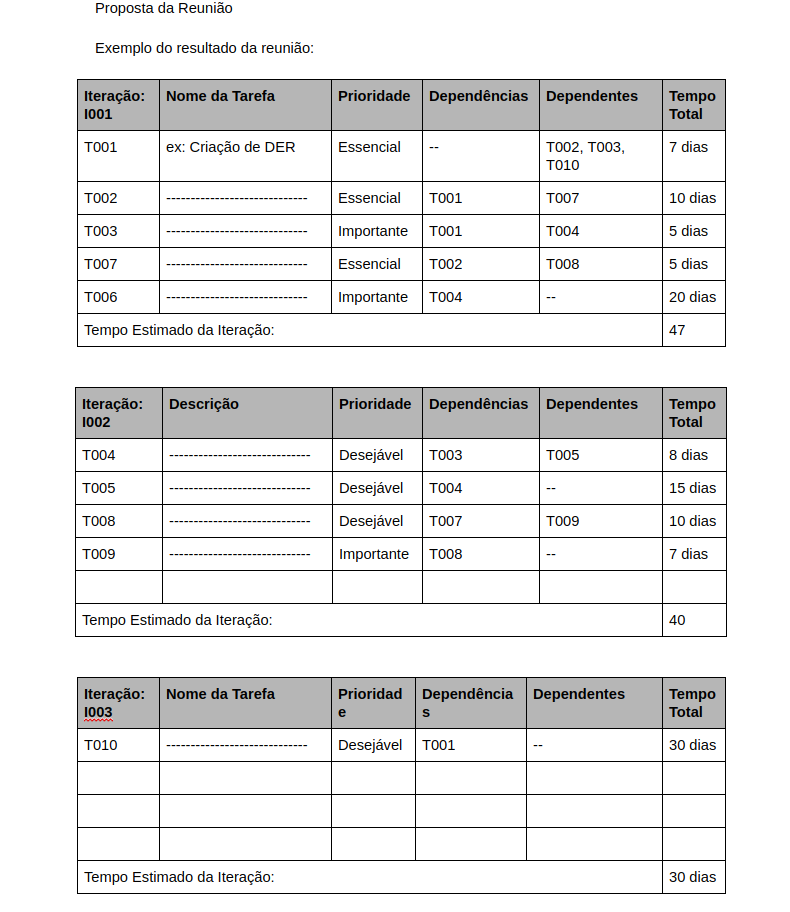
\includegraphics[width=\textwidth]{planejamento2}
	\caption{Documento de proposta de reunião}
	\label{Figura 6}
\end{figure}


\section{Referências bibliográficas}
Utilize o mendley, o jabref ou diretamente o bibtex para gerenciar suas referências biliográficas. As referências são criadas automaticamente de acordo com o uso no texto.

Exemplo: Redes de computadores, segundo \cite{t2013} é considerada..... Já \cite{kurose2010} apresenta uma versão...

Analisando os pressupostos de \cite{ref3} e \cite{ref4} concluimos que....


\renewcommand\refname{} %%Referências bibliográficas}  
\bibliographystyle{ieeetr}
\bibliography{referencias} 
\end{document}